ダウンロードURLにアクセスし、32bitシステムであればgo1.4.2.linux-386.tar.gzを、64bitシステムであればgo1.2.2.linux-amd64.tar.gzをダウンロードします。

以下ではGoがインストールされたディレクトリを\texttt{\$GO\_INSTALL\_DIR}と仮定します。

\texttt{tar.gz}をインストールディレクトリに解凍します:\texttt{tar zxvf go1.4.2.linux-amd64.tar.gz -C \$GO\_INSTALL\_DIR}

PATHを設定します。\texttt{export PATH=\$PATH:\$GO\_INSTALL\_DIR\//go\//bin}

その後、\texttt{go}を実行します。

\begin{figure}[H]
  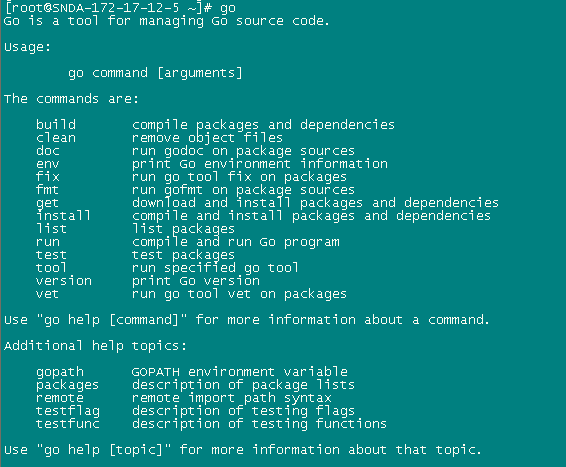
\includegraphics[width=14cm]{1.1.linux.png}
   \label{図1.2}
   \caption{Linuxシステムでインストールに成功したあとgoを実行した時に表示する情報}
\end{figure}

もしgoのUsage情報が表示された場合は、goはすでにインストールされています。もしこのコマンドが存在しないと出てきた場合は、自分のPATH環境変数の中にgoのインストールディレクトリが含まれているか確認してください。

